\documentclass[
11pt, % The default document font size, options: 10pt, 11pt, 12pt
codirector, % Uncomment to add a codirector to the title page
]{charter} 




% El títulos de la memoria, se usa en la carátula y se puede usar el cualquier lugar del documento con el comando \ttitle
\titulo{Comunicador para centrales de alarma} 

% Nombre del posgrado, se usa en la carátula y se puede usar el cualquier lugar del documento con el comando \degreename
%\posgrado{Carrera de Especialización en Sistemas Embebidos} 
%\posgrado{Carrera de Especialización en Internet de las Cosas} 
%\posgrado{Carrera de Especialización en Intelegencia Artificial}
%\posgrado{Maestría en Sistemas Embebidos} 
\posgrado{Maestría en Internet de las cosas}

% Tu nombre, se puede usar el cualquier lugar del documento con el comando \authorname
\autor{Mariano Mondani} 

% El nombre del director y co-director, se puede usar el cualquier lugar del documento con el comando \supname y \cosupname y \pertesupname y \pertecosupname
\director{Nombre del Director}
\pertenenciaDirector{pertenencia} 
% FIXME:NO IMPLEMENTADO EL CODIRECTOR ni su pertenencia
\codirector{John Doe} % para que aparezca en la portada se debe descomentar la opción codirector en el documentclass
\pertenenciaCoDirector{FIUBA}

% Nombre del cliente, quien va a aprobar los resultados del proyecto, se puede usar con el comando \clientename y \empclientename
\cliente{Claudio Bongiorno}
\empresaCliente{X-28 Alarmas}

% Nombre y pertenencia de los jurados, se pueden usar el cualquier lugar del documento con el comando \jurunoname, \jurdosname y \jurtresname y \perteunoname, \pertedosname y \pertetresname.
\juradoUno{Nombre y Apellido (1)}
\pertenenciaJurUno{pertenencia (1)} 
\juradoDos{Nombre y Apellido (2)}
\pertenenciaJurDos{pertenencia (2)}
\juradoTres{Nombre y Apellido (3)}
\pertenenciaJurTres{pertenencia (3)}
 
\fechaINICIO{30 de abril de 2021}		%Fecha de inicio de la cursada de GdP \fechaInicioName
\fechaFINALPlan{18 de junio de 2021} 	%Fecha de final de cursada de GdP
\fechaFINALTrabajo{25 de abril de 2022}	%Fecha de defensa pública del trabajo final


\begin{document}

\maketitle
\thispagestyle{empty}
\pagebreak


\thispagestyle{empty}
{\setlength{\parskip}{0pt}
\tableofcontents{}
}
\pagebreak


\section{Registros de cambios}
\label{sec:registro}


\begin{table}[ht]
\label{tab:registro}
\centering
\begin{tabularx}{\linewidth}{@{}|c|X|c|@{}}
\hline
\rowcolor[HTML]{C0C0C0} 
Revisión & \multicolumn{1}{c|}{\cellcolor[HTML]{C0C0C0}Detalles de los cambios realizados} & Fecha      \\ \hline
0      & Creación del documento\newline Se completa hasta el punto 8 inclusive, sin incluir el punto 5 &30/04/2021 \\ \hline
1      & Se corrigen errores en la Descipción, Identificación de los interesados y Alcance.\newline Se completa hasta el punto 12 inclusive.                  & 09/05/2021 \\ \hline
%2      & Se completa hasta el punto 7 inclusive
%		  Se puede agregar algo más \newline
%		  En distintas líneas \newline
%		  Así                                                    & dd/mm/aaaa \\ \hline
%3      & Se completa hasta el punto 11 inclusive                & dd/mm/aaaa \\ \hline
%4      & Se completa el plan	                                 & dd/mm/aaaa \\ \hline
\end{tabularx}
\end{table}

\pagebreak



\section{Acta de constitución del proyecto}
\label{sec:acta}

\begin{flushright}
Buenos Aires, \fechaInicioName
\end{flushright}

\vspace{2cm}

Por medio de la presente se acuerda con el Ing. \authorname\hspace{1px} que su Trabajo Final de la \degreename\hspace{1px} se titulará ``\ttitle'', consistirá esencialmente en la implementación de un sistema que permitirá comunicar una alarma domiciliaria con una aplicación móvil, y tendrá un presupuesto preliminar estimado de 600 hs de trabajo, con fecha de inicio \fechaInicioName\hspace{1px} y fecha de presentación pública \fechaFinalName.

Se adjunta a esta acta la planificación inicial.

\vfill

% Esta parte se construye sola con la información que hayan cargado en el preámbulo del documento y no debe modificarla
\begin{table}[ht]
\centering
\begin{tabular}{ccc}
\begin{tabular}[c]{@{}c@{}}Ariel Lutenberg \\ Director posgrado FIUBA\end{tabular} & \hspace{2cm} & \begin{tabular}[c]{@{}c@{}}\clientename \\ \empclientename \end{tabular} \vspace{2.5cm} \\ 
\multicolumn{3}{c}{\begin{tabular}[c]{@{}c@{}} \supname \\ Director del Trabajo Final\end{tabular}} \vspace{2.5cm} \\
%\begin{tabular}[c]{@{}c@{}}\jurunoname \\ Jurado del Trabajo Final\end{tabular}     &  & \begin{tabular}[c]{@{}c@{}}\jurdosname\\ Jurado del Trabajo Final\end{tabular}  \vspace{2.5cm}  \\
%\multicolumn{3}{c}{\begin{tabular}[c]{@{}c@{}} \jurtresname\\ Jurado del Trabajo Final\end{tabular}} \vspace{.5cm}                                                                     
\end{tabular}
\end{table}




\section{Descripción técnica-conceptual del proyecto a realizar}
\label{sec:descripcion}

%\begin{consigna}{black} 

Desde hace más de una década es común encontrar en un sistema de alarma hogareño algún tipo de comunicador. Estos, generalmente, permiten recibir avisos cuando se produce un evento en la alarma como enviarle comandos para que se realice alguna acción en el sistema.

Con el paso de los años la forma de conexión entre el usuario y su alarma ha cambiado. Comenzó siendo a través de la línea telefónica, para luego, pasar a llevarse a cabo mediante la red celular. 

Durante muchos años los usuarios percibieron como ágil y novedosa la comunicación a través de mensajes de texto (SMS). El comunicador le enviaba un mensaje cuando se producía algún evento en la alarma y el usuario podía realizar una acción enviando comandos sencillos. Sin embargo, la comunicación mediante SMS fue quedando obsoleta en la vida cotidiana y por lo tanto comenzó a ser considerado un medio poco confiable de interacción con un sistema de seguridad.

Impulsada por esta situación, la empresa comenzó a orientar sus esfuerzos a desarrollar nuevos productos que les permitan a los usuarios relacionarse con sus equipos de una forma más sencilla, consistente y robusta.

En este contexto surge el presente proyecto: un equipo que se conecta al sistema de alarma como cualquier otro dispositivo y que es acompañado mediante una aplicación que permite conocer el estado de la alarma, recibir eventos y enviar comandos.

A pesar de que actualmente la competencia de X-28 Alarmas ofrece comunicadores compatibles con las centrales de alarma de la marca, el principal diferencial que va a ofrecer este nuevo producto es la posibilidad de acceder a una gran variedad de funcionalidades del sistema de seguridad. 

Esto se debe a que los comunicadores universales solo ofrecen un conjunto muy limitado de funciones, generalmente activar y desactivar la central, recibir notificaciones cuando el sistema está sonando y, en algunos casos, manejar una o dos cargas eléctricas. En cambio, el producto propuesto, busca cubrir una más amplia gama de necesidades:

\begin{itemize}
	\item Asociar múltiples alarmas a un mismo usuario, con distintos niveles de acceso.
	\item Conocer el estado de cada uno de los sensores que componen la alarma.
	\item Permitir asignarle un nombre distintivo a cada: alarma, sensor, usuario y carga eléctrica.
	\item Recibir notificaciones no solo por disparos en la alarma, sino también por problemas en la red eléctrica, por activación o desactivación del sistema distinguiendo qué usuario lo hizo, por eventos personalizados, etc.
	\item Ser compatible con la línea de productos de automatización de X-28 Alarmas.
\end{itemize}

Además del equipo que va a ser conectado en la alarma y de la aplicación utilizada por el usuario, el sistema propuesto en este proyecto se completa con el desarrollo de un backend que permita la comunicación entre alarmas y usuarios. 

En la Figura \ref{fig:diagBloques} se muestra el diagrama en bloques del sistema. Como puede verse, el comunicador se va a conectar a Internet mediante dos posibles vías: Wi-Fi o red celular. Al contemplar dos formas de conexión, no solo se otorga mayor robustez a la comunicación, sino también se cubre una mayor variedad de casos de uso. Este equipo podría ser usado mediante Wi-Fi en el caso en el que la cobertura celular, en el lugar de la instalación, sea deficiente o en el caso en el que el usuario no quiera atarse a un abono mensual en relación al servicio celular. Por el contrario, podría ser utilizado a través de la red celular en aquellas situaciones en donde no hay una red Wi-Fi disponible.

%\vspace{25px}

\begin{figure}[htpb]
\centering 
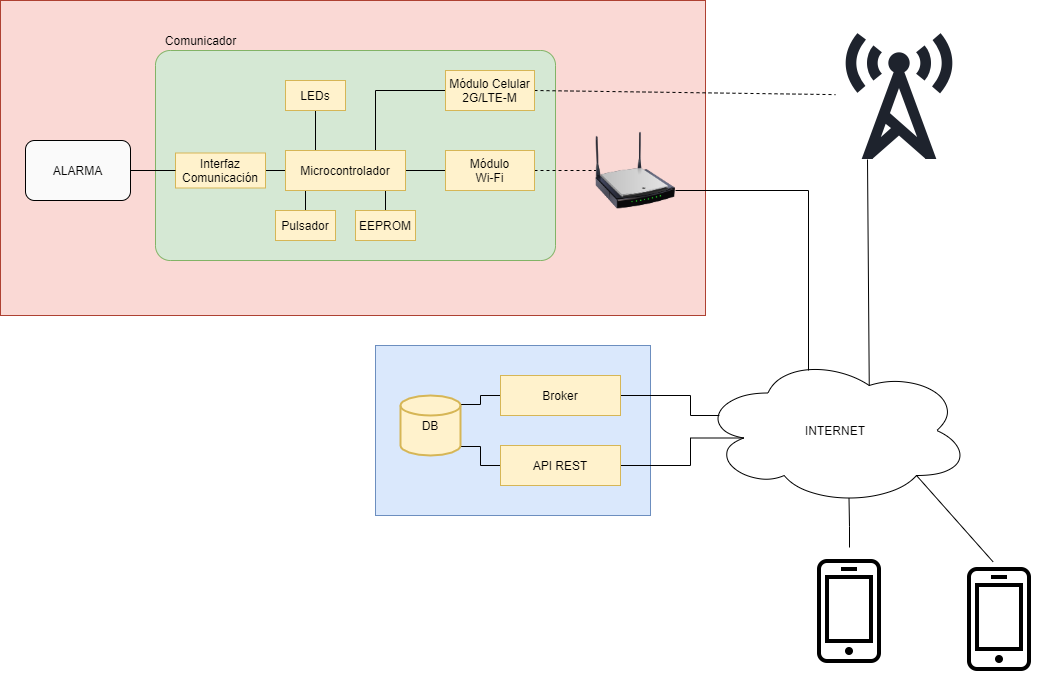
\includegraphics[width=\textwidth]{./Figuras/diagBloques.png}
\caption{Diagrama en bloques del sistema}
\label{fig:diagBloques}
\end{figure}

\vspace{25px}

Finalmente, en la Figura \ref{fig:diagBloques} se observa que el backend se compone de:

\begin{itemize}
	\item Un broker que se encarga de la comunicación entre las apps de los usuarios finales y los comunicadores
	\item Una API de tipo REST utilizada por las apps para: login, obtener información de la alarma, enviar comandos al comunicador, etc.
	\item Una base de datos en donde se lleva un registro de los comunicadores, los usuarios de las apps y el estado y configuración de cada uno de los sistemas de alarma.
\end{itemize}

%\end{consigna}


\section{Identificación y análisis de los interesados}
\label{sec:interesados}

%\begin{consigna}{black} 

\begin{table}[H]
%\caption{Identificación de los interesados}
%\label{tab:interesados}
\begin{tabularx}{\linewidth}{@{}|l|X|X|X|@{}}
\hline
\rowcolor[HTML]{C0C0C0} 
Rol           & Nombre y Apellido & Organización 	& Puesto 	\\ \hline
Auspiciante   & Norberto Vergani      &\empclientename	& Director       	\\ \hline
Cliente e impulsor      & \clientename      &\empclientename	& Jefe de área       	\\ \hline
Responsable   & \authorname       & FIUBA        	& Alumno 	\\ \hline
Colaboradores & Pablo Marchant \newline
			   Docentes CEIoT   & \empclientename \newline
			   					FIUBA             & Jefe de área\newline
			   									  -       	\\ \hline
Orientador    & \supname	      & \pertesupname 	& Director Trabajo final \\ \hline
Usuario final & Clientes de X-28 Alarmas & -             	& -       	\\ \hline
\end{tabularx}
\end{table}


\begin{itemize}
	\item Auspiciante: busca completar la línea de productos de seguridad comercializados por la
empresa. Está interesado en que el proyecto se complete en el tiempo establecido y está dispuesto a invertir para ayudar a lograrlo. Además tiene una amplia experiencia en el diseño de hardware de sistemas embebidos y en la programación de firmware. Se deben aprovechar especialmente sus conocimientos en este último tema.\\
Debido a ser una empresa que vende productos de seguridad, se pone especial atención en mantener el prestigio y la confianza que los clientes depositan en la empresa, por lo que es exigente en cuanto a la calidad y confiabilidad del producto.
	\item Cliente e impulsor: es exigente en cuanto a la integración de los nuevos dispositivos con la línea actual de productos. Su objetivo es que los nuevos equipos sean confiables y robustos en cuanto a su usabilidad. Además cuenta con conocimientos en el diseño de hardware y a participado en el diseño e implementación de gran parte de los productos actuales de la empresa. Sus sugerencias van a ayudar en el diseño del circuito impreso.
	\item Colaboradores: Pablo Marchant es el jefe del área de Comercio exterior, y va a ser el encargado de conseguir muchos de los componentes necesarios para el hardware. Su colaboración va a permitir encontrar la forma de reducir los costos en los componentes electrónicos.
	\item Usuario final: los clientes de X-28 Alarmas estás acostumbrados a que los productos de la marca sean sencillos de utilizar. Además, buscan que los nuevos productos que se ofrecen sean compatibles con los ya existentes, permitiéndoles agregarlos sin problemas a sus sistemas de alarma.
\end{itemize}

%\end{consigna}



\section{1. Propósito del proyecto}
\label{sec:proposito}

%\begin{consigna}{red}
El propósito de este proyecto consiste en diseñar e implementar un comunicador, una aplicación y un backend que le permita a los usuarios de las alarmas de X-28 comunicarse con sus sistemas de seguridad. Se busca lograr, por un lado, un producto que no solo sea sencillo de utilizar sino también robusto y seguro. Por otro lado, a lo largo del proyecto, se buscarán introducir prácticas de programación y periféricos de hardware que puedan ser reutilizados en otros proyectos  y por lo tanto aumenten la base de conocimiento del sector de Investigación y Desarrollo.
%\end{consigna}

\section{2. Alcance del proyecto}
\label{sec:alcance}

%\begin{consigna}{red}

El proyecto incluye:

\begin{itemize}
	\item El desarrollo de un sistema embebido capaz de conectarse a un sistema de alarma y a Internet, mediante Wi-Fi y red celular. Se incluye tanto hardware como firmware.
	\item El desarrollo del prototipo de una aplicación híbrida (probada en Android) para poder controlar las alarmas
	\item El diseño del modelo de datos utilizado en la base de datos del backend
	\item El desarrollo de un broker que permita la comunicación entre las aplicaciones y los comunicadores.
	\item El desarrollo de una API REST que le permita a las aplicaciones obtener datos de las alarmas y enviarles comandos
\end{itemize}

El proyecto no incluye:

\begin{itemize}
	\item Diseño del gabinete para el comunicador.
	\item Las implementaciones particulares para que la aplicación funcione en iOS.
	\item Consideraciones de diseño para el despliegue del broker y la API en un entorno cloud, contemplando alta disponibilidad y escalamiento.
\end{itemize}

%\end{consigna}


\section{3. Supuestos del proyecto}
\label{sec:supuestos}

%\begin{consigna}{red}
Para el desarrollo del presente proyecto se supone que:

\begin{itemize}
	\item Se podrá diseñar e implementar el producto, logrando su correcto funcionamiento.
	\item No habrá dificultades para conseguir los componentes electrónicos necesarios.
	\item Se contará con los conocimientos necesarios para desarrollar la aplicación híbrida y el backend. En caso de no contar con ciertos conocimientos, se los podrá investigar y aplicar satisfactoriamente.
	\item Dentro de la lista de proyectos actualmente en curso del área de Investigación y Desarrollo, se le dará la dedicación suficiente al presente proyecto y no se lo suspenderá en favor del desarrollo de otros productos.
\end{itemize}

%\end{consigna}

\section{4. Requerimientos}
\label{sec:requerimientos}

%\begin{consigna}{red}

\begin{enumerate}
	\item Requerimientos del hardware
		\begin{enumerate}
			\item Incluir una interfaz sencilla con el usuario. Debe existir un único pulsador para que el usuario realice acciones relacionadas con la red Wi-Fi.
			\item Incluir un led bicolor (rojo y verde) para señalizar el estado de funcionamiento y de error.
			\item Incluir una interfaz que permita conectar el comunicador al bus del sistema de alarma.
			\item Tener una memoria EEPROM para almacenar información de configuración.
			\item Tener un módulo Wi-Fi
			\item Tener un módulo celular pueda conectarse a la red celular de 2G y de 4G Cat M1.
			\item El PCB debe respetar las dimensiones del gabinete en el que va a ser comercializado el comunicador.
		\end{enumerate}
	\item Requerimientos del software embebido
		\begin{enumerate}
			\item Configuración de la red Wi-Fi a la que conectarse mediante WPS.
			\item Configuración de la red Wi-Fi a la que conectarse mediante la app.
			\item Interpretar los comandos AT del módulo celular.
			\item Implementar el protocolo definido para comunicar los comunicadores y el broker.
			\item La conexión con el broker debe ser implementada con TLS.
			\item La conexión con el broker se debe mantener abierta permanentemente.
			\item Ser compatible con el protocolo de comunicación de las alarmas de X-28.
			\item Guardar en la memoria EEPROM la configuración para el correcto funcionamiento del comunicador.
			\item Implementar la lógica necesaria para elegir prioritariamente la conexión con el broker mediante Wi-Fi y en caso de fallar, hacerlo mediante la red celular.
		\end{enumerate}
	\item Requerimientos del protocolo de comunicación entre dispositivos y el broker
		\begin{enumerate}
			\item Definir la forma en la que se van a identificar los dispositivos a nivel lógico con el broker.
			\item Permitir autenticar al dispositvo.
			\item Incluir una lógica de keepalive.
			\item Permitir solicitar fecha y hora en función de la región en la que esté el comunicador.
			\item Implementar comandos para solicitarle información al comunicador.
			\item Permitir el envío de eventos cuando ocurre un suceso en el sistema de alarma.
			\item Permitir enviar comandos al comunicador para realizar acciones en la alarma.
		\end{enumerate}
	\item Requerimiento de la aplicación híbrida
		\begin{enumerate}
			\item Incluir un login.
			\item Proceso guiado para ayudar a configurar la red Wi-Fi a la que se va a conectar el comunicador.
			\item Cada usuario de la aplicación puede agregar múltiples alarmas para gestionarlas.
			\item Mostrar el estado de la alarma (activada, desactivada, sonando) y problemas que pueda presentar (batería baaja, red eléctrica cortada, error de comunicación, etc).
			\item Permitir enviar comandos a la alarma: activar, desactivar, cambiar su modo, disparar manualmente, incluir y excluir sensores, etc.
			\item Mostrar el estado de cada uno de los sensores.
			\item Mostrar el estado de cada una de las cargas eléctrica de la alarma y permitir encenderlas o apagarlas.
			\item Incluir el CRUD de los sensores que tiene la alarma.
			\item Incluir el CRUD de las cargas eléctricas que maneja la alarma.
			\item Incluir el CRUD de los usuarios que tiene la alarma.
		\end{enumerate}
	\item Requerimientos del broker
		\begin{enumerate}
			\item Permitir múltiples comunicadores conectados simultáneamente.
			\item Interpretar la información que llega desde los comunicadores para actualizar la información en la base de datos.
			\item Reenviar los mensajes que llegan desde las aplicaciones móviles a los comunicadores.
			\item Enviar notificaciones push a las aplicaciones cuando se produzcan eventos en los comunicadores que tienen asociados.
		\end{enumerate}
	\item Requerimientos de la API REST
		\begin{enumerate}
			\item Todos los endpoints deben incluir un token exclusivo para cada aplicación.
			\item Implementar un endpoint para que las aplicaciones puedan autenticarse.
			\item Incluir endpoints para solicitar información de los comunicadores.
			\item Incluir endpoints para realizar el CRUD de comunicadores
			\item Incluir endpoints para realizar el CRUD de los sensores de una alarma
			\item Incluir endpoints para realizar el CRUD de las usuarios de una alarma
			\item Incluir endpoints para realizar el CRUD de las cargas eléctricas de una alarma
			\item Incluir endpoints para enviar comandos a los comunicadores.
		\end{enumerate}
	\item Requerimientos de la base de datos
		\begin{enumerate}
			\item Persistir los identificadores de los comunicadores que fueron fabricados.
			\item Persistir la información de los usuarios de las aplicaciones y qué comunicadores tienen asociados.
			\item Persistir la información del estado de cada alarma: estado de cada sensor, estado de la red eléctrica, estado de la batería; nombres de los sensores, usuarios y cargas eléctricas.
		\end{enumerate}

\end{enumerate}

%\end{consigna}

\section{5. Historias de usuarios (\textit{Product backlog})}
\label{sec:backlog}

\begin{consigna}{red}
Descripción: En esta sección se deben incluir las historias de usuarios y su ponderación (\textit{history points}). Recordar que las historias de usuarios son descripciones cortas y simples de una característica contada desde la perspectiva de la persona que desea la nueva capacidad, generalmente un usuario o cliente del sistema. La ponderación es un número entero que representa el tamaño de la historia comparada con otras historias de similar tipo.

Se debe indicar explícitamente el criterio para calcular los \textit{story points} de cada historia
\end{consigna}

\section{6. Entregables principales del proyecto}
\label{sec:entregables}

%\begin{consigna}{red}

\begin{itemize}
	\item Comuninicador según requerimientos y diagrama esquemático.
	\item Prototipo funcional de la aplicación híbrida funcionando en Android.
	\item Implementación del modelo de datos en la base de datos.
	\item Implementación del broker.
	\item Implementación de la API REST.
	\item Informe de avance.
	\item Memoria escrita del proyecto.
	\item Presentación publica y defensa del trabajo ante el jurado.
\end{itemize}

%\end{consigna}

\section{7. Desglose del trabajo en tareas}
\label{sec:wbs}

%\begin{consigna}{red}

\begin{enumerate}
	\item Investigación preliminar (65 horas)
		\begin{enumerate}
			\item Investigación acerca de los posibles módulos Wi-Fi y elección de uno de ellos (10 horas)
			\item Investigación acerca de los posibles módulos celulares y elección de uno de ellos (10 horas)
			\item Elección del microcontrolador a usar y familiarización con el mismo (15 horas)
			\item Desarrollo del protocolo de comunicación entre los comunicadores y el broker (30 horas)
		\end{enumerate}
	\item Desarrollo del hardware (60 horas)
		\begin{enumerate}
			\item Diseño del diagrama esquemático y determinación del BOM (20 horas)
			\item Diseño del PCB y fabricación de un prototipo (30 horas)
			\item Verificación del prototipo (10 horas)
		\end{enumerate}
	\item Desarrollo del firmware (230 horas)
		\begin{enumerate}
			\item Implementación del driver para el módulo Wi-Fi (30 horas)
			\item Testeo del driver para el módulo Wi-Fi (10 horas)
			\item Implementación del driver para el módulo celular (30 horas)
			\item Testeo del driver para el módulo celular (10 horas)
			\item Implementación de la capa de comunicación con el sistema de alarma (40 horas)
			\item Testeo de la capa de comunicación con la alarma (10 horas)
			\item Implementación del protocolo de comunicación con el broker (20 horas)
			\item Testeo del protocolo de comunicación con el broker (5 horas)
			\item Programación de la aplicación principal e integración de los drivers (60 horas)
			\item Testeo del firmware (15 horas)
		\end{enumerate}
	\item Desarrollo del backend (85 horas)
		\begin{enumerate}
			\item Definición del modelo de datos para la base de datos (5 horas)
			\item Implementación del broker (30 horas)
			\item Testeo del broker (10 horas)
			\item Implementación de la API REST (20 horas)
			\item Testeo de la API REST (10 horas)
			\item Integración entre el comunicador y el broker (10 horas)
		\end{enumerate}
	\item Desarrollo de la aplicación híbrida (160 horas)
		\begin{enumerate}
			\item Profundización de los conocimientos para el desarrollo de la aplicación (25 horas)
			\item Maquetado de la aplicación (20 horas)
			\item Implementación de la aplicación (90 horas)
			\item Testeo de la aplicación (10 horas)
			\item Integración entre la aplicación y el backend (15 horas)
		\end{enumerate}
	\item Presentación del proyecto (70 horas)
		\begin{enumerate}
			\item Escritura del informe de avance (15 horas)
			\item Escritura del informe final (40 horas)
			\item Escritura de la presentación pública (15 horas)
		\end{enumerate}
\end{enumerate}

Cantidad total de horas: 670 horas

%\end{consigna}

\section{8. Diagrama de Activity On Node}
\label{sec:AoN}


\begin{figure}[htpb]
\centering 
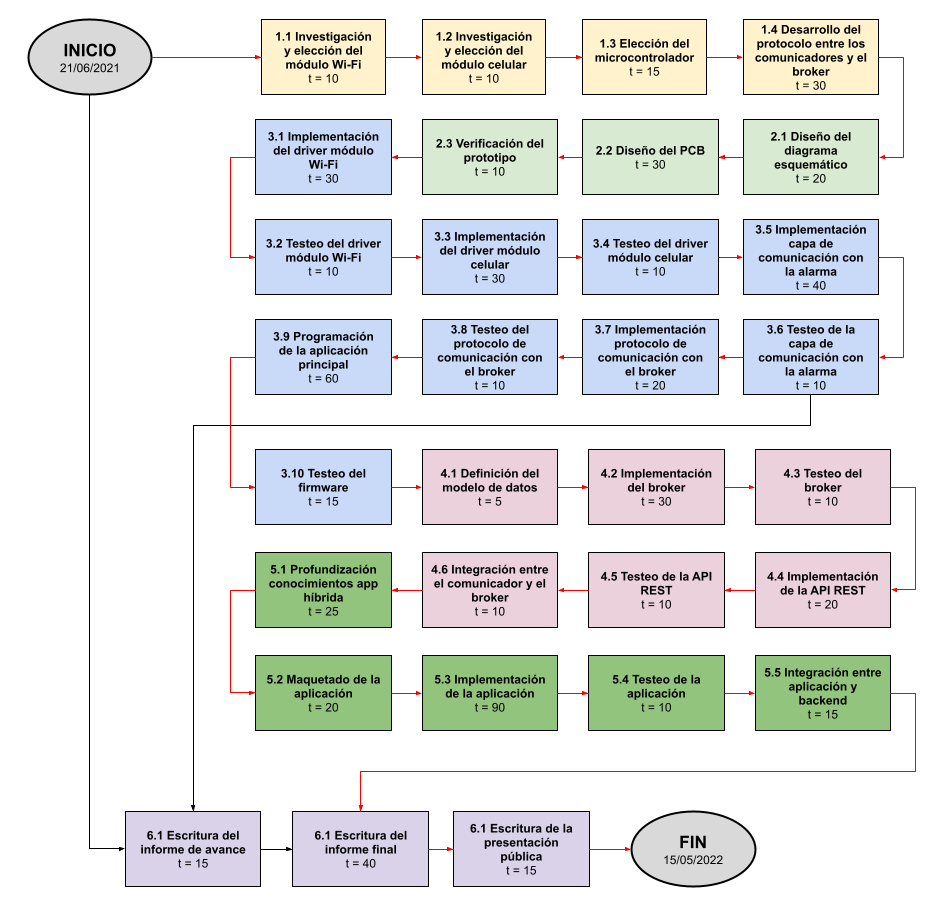
\includegraphics[width=\textwidth]{./Figuras/AoN.png}
\caption{Diagrama en \textit{Activity on Node}}
\label{fig:AoN}
\end{figure}

Los tiempos están expresados en horas.



\section{9. Diagrama de Gantt}
\label{sec:gantt}

%\begin{consigna}{red}

\begin{figure}[htpb]
\centering 
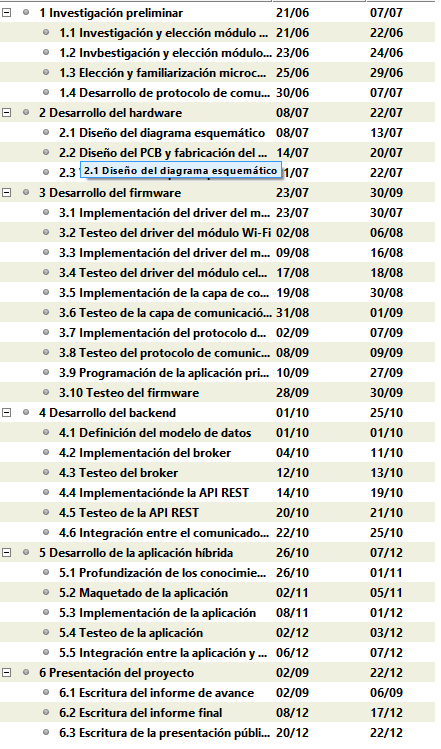
\includegraphics[width=.75\textwidth]{./Figuras/gantt1.png}
\caption{Diagrama de Gantt: lista de tareas}
\label{fig:gantt1}
\end{figure}

\begin{figure}[htpb]
\centering 
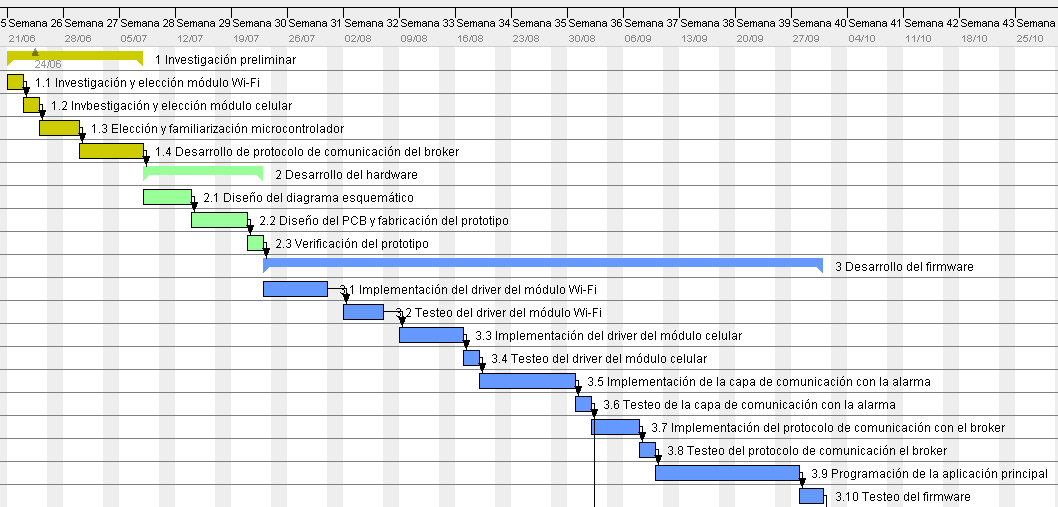
\includegraphics[width=\textwidth]{./Figuras/gantt2.png}
\caption{Detalle del diagrama de Gantt}
\label{fig:gantt2}
\end{figure}

\begin{figure}[htpb]
\centering 
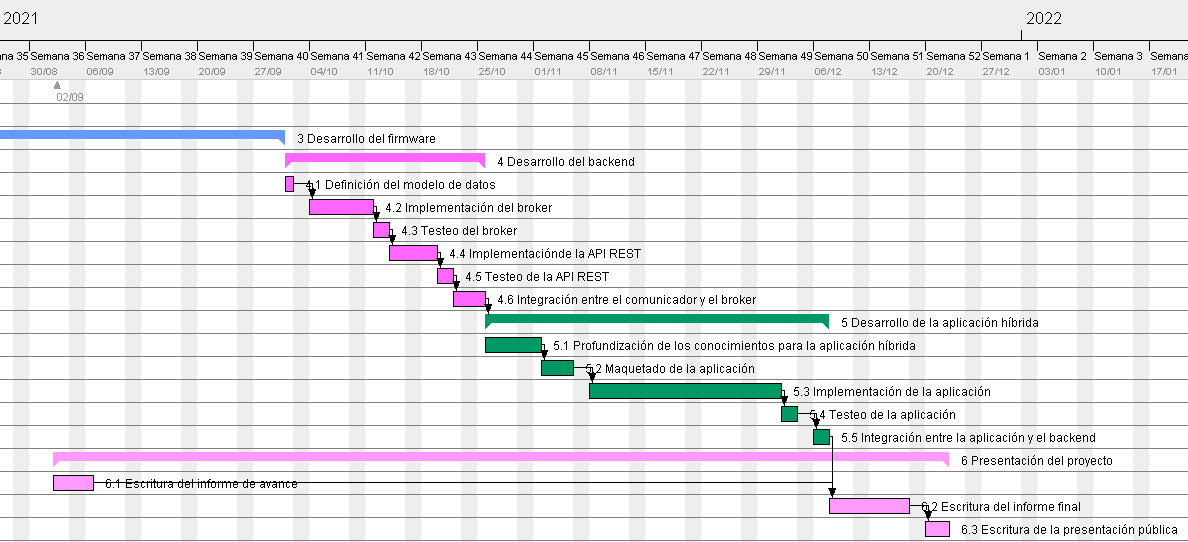
\includegraphics[width=\textwidth]{./Figuras/gantt3.png}
\caption{Detalle del diagrama de Gantt}
\label{fig:gantt3}
\end{figure}

%\end{consigna}


\section{10. Presupuesto detallado del proyecto}
\label{sec:presupuesto}

%\begin{consigna}{red}


%\end{consigna}

\begin{table}[htpb]
\centering
\begin{tabularx}{\linewidth}{@{}|X|c|r|r|@{}}
\hline
\rowcolor[HTML]{C0C0C0} 
\multicolumn{4}{|c|}{\cellcolor[HTML]{C0C0C0}COSTOS DIRECTOS} \\ \hline
\rowcolor[HTML]{C0C0C0} 
Descripción &
  \multicolumn{1}{c|}{\cellcolor[HTML]{C0C0C0}Cantidad} &
  \multicolumn{1}{c|}{\cellcolor[HTML]{C0C0C0}Valor unitario} &
  \multicolumn{1}{c|}{\cellcolor[HTML]{C0C0C0}Valor total} \\ \hline
 Trabajo directo &
  \multicolumn{1}{c|}{670} &
  \multicolumn{1}{c|}{\$700} &
  \multicolumn{1}{c|}{\$469.000} \\ \hline
 Placa de desarrollo &
  \multicolumn{1}{c|}{1} &
  \multicolumn{1}{c|}{\$7.000} &
  \multicolumn{1}{c|}{\$7.000} \\ \hline
 Fabricación del PCB &
  \multicolumn{1}{c|}{1} &
  \multicolumn{1}{c|}{\$5.000} &
  \multicolumn{1}{c|}{\$5.000} \\ \hline
\multicolumn{3}{|c|}{SUBTOTAL} &
  \multicolumn{1}{c|}{\$481.000} \\ \hline
\rowcolor[HTML]{C0C0C0} 
\multicolumn{4}{|c|}{\cellcolor[HTML]{C0C0C0}COSTOS INDIRECTOS} \\ \hline
\rowcolor[HTML]{C0C0C0} 
Descripción &
  \multicolumn{1}{c|}{\cellcolor[HTML]{C0C0C0}Cantidad} &
  \multicolumn{1}{c|}{\cellcolor[HTML]{C0C0C0}Valor unitario} &
  \multicolumn{1}{c|}{\cellcolor[HTML]{C0C0C0}Valor total} \\ \hline
\multicolumn{1}{|l|}{Costos indirectos (30\% del trabajo directo)} &
   - &
   - &
   \$140.700\\ \hline

\multicolumn{3}{|c|}{SUBTOTAL} &
  \multicolumn{1}{c|}{\$140.700} \\ \hline
\rowcolor[HTML]{C0C0C0}
\multicolumn{3}{|c|}{TOTAL} &
   \$621.700\\ \hline
\end{tabularx}%
\end{table}


\section{11. Matriz de asignación de responsabilidades}
\label{sec:responsabilidades}
%\begin{consigna}{red}

\begin{table}[htpb]
\centering
\resizebox{\textwidth}{!}{%
\begin{tabular}{|c|c|c|c|c|c|}
\hline
\rowcolor[HTML]{C0C0C0} 
\cellcolor[HTML]{C0C0C0} &
  \cellcolor[HTML]{C0C0C0} &
  \multicolumn{4}{c|}{\cellcolor[HTML]{C0C0C0}Listar todos los nombres y roles del proyecto} \\ \cline{3-6} 
\rowcolor[HTML]{C0C0C0} 
\cellcolor[HTML]{C0C0C0} &
  \cellcolor[HTML]{C0C0C0} &
  Responsable &
  Orientador &
  Auspiciante &
  Cliente \\ \cline{3-6} 
\rowcolor[HTML]{C0C0C0} 
\multirow{-3}{*}{\cellcolor[HTML]{C0C0C0}\begin{tabular}[c]{@{}c@{}}Código\\ WBS\end{tabular}} &
  \multirow{-3}{*}{\cellcolor[HTML]{C0C0C0}Nombre de la tarea} &
  \authorname &
  \supname &
  Norberto Vergani &
  \clientename \\ \hline
 1 & Investigación preliminar & P & I & C & A \\ \hline
 2 & Desarrollo del hardware & P & I & I & C/A \\ \hline
 3 & Desarrollo del firmware & P & C & A & I \\ \hline
 4 & Desarrollo del backend & P & C & I & A \\ \hline
 5.1 & Profundización de los conocimientos & P & C & - & - \\ \hline
 5.2 & Maquetado de la app & P & I & I & A \\ \hline
 5.3 & Implementación de la app & P & C & I & A \\ \hline
 5.4 & Testeo de la app & P & - & I & I \\ \hline
 5.5 & Integración & P & I & I & A \\ \hline
 6 & Presentación del proyecto & P & A & - & - \\ \hline
\end{tabular}%
}
\end{table}

{\footnotesize
Referencias:
\begin{itemize}
	\item P = Responsabilidad Primaria
	\item S = Responsabilidad Secundaria
	\item A = Aprobación
	\item I = Informado
	\item C = Consultado
\end{itemize}
} %footnotesize

%\end{consigna}

\section{12. Gestión de riesgos}
\label{sec:riesgos}

%\begin{consigna}{red}

Riesgo 1:pérdida del prototipo del comunicador.
\begin{itemize}
	\item Severidad (7): al contar con un único prototipo, en caso de producirse un daño irreparable, el proyecto se detiene hasta que se construya uno nuevo.
	\item Probabilidad de ocurrencia (4): se toman los recaudos necesarios para evitar dañar el prototipo
\end{itemize}   

Riesgo 2: imposibilidad de conseguir componentes electrónicos clave.
\begin{itemize}
	\item Severidad (7): los componentes de mayor importancia son el módulo Wi-Fi y el módulo celular. En caso de no conseguir los componentes elegidos, tanto el PCB como el firmware se verán seriamente afectados. 
	\item Ocurrencia (2): la empresa cuenta con varios proveedores de componentes, por lo que es difícil no poder conseguirlos.
\end{itemize}

Riesgo 3: retraso en la fabricación del PCB
\begin{itemize}
	\item Severidad (6): un retraso en la fabricación retrasaría el desarrollo del firmware y por lo tanto el del backend y el de la app.
	\item Ocurrencia (2): de acuerdo a la experiencia que se tiene con el proveedor de PCB, se concluye que en raras ocasiones se produjo un retraso y, en caso de ocurrir, fue un retraso de unos pocos días.
\end{itemize}

Riesgo 4: el proyecto queda suspendido frente a otros proyectos más prioritarios.
\begin{itemize}
	\item Severidad (10): una decisión por parte del directorio que implique suspender este proyecto debido a que hay otros más prioritarios puede provocar que no se puedan cumplir con los plazos establecidos en esta planificación.
	\item Ocurrencia (2): debido al fuerte interés de la empresa por completar su oferta de productos con este tipo de comunicadores, es difícil pensar que se vaya a dejar de lado este proyecto.
\end{itemize}

Riesgo 5: retrasos en la implementación de la app
\begin{itemize}
	\item Severidad (8): una demora en la implementación de la app que acompaña al comunicador retrasaría la salida del producto.
	\item Ocurrencia (5): debido al bajo dominio que se tiene en relación al desarrollo de aplicaciones híbridas, pueden aparecer demoras debido a problemas con la implementación.
\end{itemize}


Tabla de gestión de riesgos:      (El RPN se calcula como RPN=SxO)

\begin{table}[htpb]
\centering
\begin{tabularx}{\linewidth}{@{}|X|c|c|c|c|c|c|@{}}
\hline
\rowcolor[HTML]{C0C0C0} 
Riesgo & S & O & RPN & S* & O* & RPN* \\ \hline
   1. Pérdida del prototipo    & 7  & 4  &  28   &  2  &  2  &   4   \\ \hline
   2. Imposibilidad de conseguir componentes   & 7  & 2  &  14   &    &    &      \\ \hline
   3. Retraso en la fabricación del PCB   & 6  & 2  &  12   &    &    &      \\ \hline
   4. Suspensión del proyecto   & 10  & 2  & 20   &    &    &      \\ \hline
   5. Retrasos en la implementación de la app   & 8  & 5  &  40   & 4   & 2   &  8    \\ \hline
\end{tabularx}%
\end{table}

Criterio adoptado: 
Se tomarán medidas de mitigación en los riesgos cuyos números de RPN sean mayores a 25.

Nota: los valores marcados con (*) en la tabla corresponden luego de haber aplicado la mitigación.

Plan de mitigación de los riesgos que originalmente excedían el RPN máximo establecido:
 
Riesgo 1: encargar varias muestras del PCB y armar varios prototipos
\begin{itemize}
  \item Severidad (2): en caso de dañarse el primer prototipo, inmediatamente se lo puede reemplazar por otro. Sin embargo, se debe minimizar la repetición de esta situación para evitar que otros miembros del equipo de Desarrollo pierdan tiempo en armar más prototipos.
  \item Probabilidad de ocurrencia (2): es difícil que, debido a una mala manipulación, se dañe más de un prototipo.
\end{itemize}

Riesgo 5: anticiparse a la etapa del proyecto relacionada con la implementación de la app e ir haciendo pruebas de concepto de distintos aspectos de la aplicación,  para profundizar los conocimientos necesarios.
\begin{itemize}
  \item Severidad (4): las posibles demoras se van a reducir ya que se va a contar con un conocimiento más profundo del framework a usar.
  \item Probabilidad de ocurrencia (2): a pesar de que, tal vez, no se llegue a la etapa de implementar la app con todos los conocimientos necesarios, la cantidad de incertidumbres respecto al framework a usar va a ser menor. 
\end{itemize} 

%\end{consigna}


\section{13. Gestión de la calidad}
\label{sec:calidad}

\begin{consigna}{red}
Para cada uno de los requerimientos del proyecto indique:
\begin{itemize} 
\item Req \#1: copiar acá el requerimiento.

\begin{itemize}
	\item Verificación para confirmar si se cumplió con lo requerido antes de mostrar el sistema al cliente. Detallar 
	\item Validación con el cliente para confirmar que está de acuerdo en que se cumplió con lo requerido. Detallar  
\end{itemize}

\end{itemize}

Tener en cuenta que en este contexto se pueden mencionar simulaciones, cálculos, revisión de hojas de datos, consulta con expertos, mediciones, etc.  Las acciones de verificación suelen considerar al entregable como ``caja blanca'', es decir se conoce en profundidad su funcionamiento interno.  En cambio, las acciones de validación suelen considerar al entregable como ``caja negra'', es decir, que no se conocen los detalles de su funcionamiento interno.

\end{consigna}


\section{14. Procesos de cierre}    
\label{sec:cierre}

\begin{consigna}{red}
Establecer las pautas de trabajo para realizar una reunión final de evaluación del proyecto, tal que contemple las siguientes actividades:

\begin{itemize}
	\item Pautas de trabajo que se seguirán para analizar si se respetó el Plan de Proyecto original:
	 - Indicar quién se ocupará de hacer esto y cuál será el procedimiento a aplicar. 
	\item Identificación de las técnicas y procedimientos útiles e inútiles que se emplearon, y los problemas que surgieron y cómo se solucionaron:
	 - Indicar quién se ocupará de hacer esto y cuál será el procedimiento para dejar registro.
	\item Indicar quién organizará el acto de agradecimiento a todos los interesados, y en especial al equipo de trabajo y colaboradores:
	  - Indicar esto y quién financiará los gastos correspondientes.
\end{itemize}

\end{consigna}


\end{document}
